\documentclass{beamer}
\mode<presentation>
{
  \usetheme{ldv}
  \setbeamercovered{transparent}
}

% Uncomment this if you're giving a presentation in german...
%\usepackage[ngerman]{babel}

% ...and rename this to "Folie"
\newcommand{\slidenomenclature}{Slide}


\usepackage[utf8]{inputenc}
\usepackage{amsmath,amssymb,amsfonts}
\usepackage{times}
\usepackage{graphicx}
\usepackage{fancyvrb}
\usepackage{array}
\usepackage{colortbl}
\usepackage{tabularx}

\definecolor{C0}{HTML}{1f77b4}
\definecolor{C1}{HTML}{ff7f0e}
\definecolor{C2}{HTML}{2ca02c}
\definecolor{C3}{HTML}{d62728}
\definecolor{C4}{HTML}{9467bd}
\definecolor{C5}{HTML}{8c564b}
\definecolor{C6}{HTML}{e377c2}
\definecolor{C7}{HTML}{7f7f7f}
\definecolor{C8}{HTML}{bcbd22}
\definecolor{C9}{HTML}{17becf}


\usepackage{pgfplots}
\usepackage{tikz}
\usetikzlibrary{calc}
\usetikzlibrary{matrix}
\usetikzlibrary{ decorations.markings}
\usetikzlibrary {decorations.shapes}
\usetikzlibrary {shapes.arrows}
\usetikzlibrary{calc}
\usetikzlibrary{matrix}
\usetikzlibrary{ decorations.markings}
\usetikzlibrary {decorations.shapes}


%Standard settings for the stage4s
\tikzset{
	style_stage/.style={
		color=black!80, %line color
		draw,
		fill=white,
		line width=1pt,
	}
}

%special parametres for stages
\tikzset{fontmatrices/.initial=\small}
\tikzset{boxsize/.initial=9mm} %Note: width=height=2*boxsize
%psoition of arrow
\tikzset{posarr/.initial=0.5}

%line style for the signals
\tikzstyle{signal} = [line width=1.5pt]%[very thick]

%line style for drawing connections
\tikzset{signalflow/.style={signal,
		decoration={markings,mark=at position \pgfkeysvalueof{/tikz/posarr} with {\arrow{>}}},postaction={decorate}}}

%set the standard parameters for A,B,C,D
\tikzset{A/.initial=$A_{}$}
\tikzset{B/.initial=$B_{}$}
\tikzset{C/.initial=$C_{}$}
\tikzset{D/.initial=$D_{}$}


%Some internal definitions
\def\rel_i_stage{0.65} %distance of the connections for B and C, is a fraction of boxsize
\def\shadesize{2pt}

%some shorthanfds for convenience
\def\boxsize{\pgfkeysvalueof{/tikz/boxsize}}

\makeatletter
\pgfdeclareshape{stagebox}{
	%anchors
	\anchor{center}{\pgf@x=0cm \pgf@y=0cm}
	\anchor{south}{\pgf@x=0cm \pgf@y=-\boxsize}
	\anchor{east}{\pgf@x=\boxsize \pgf@y=0cm}
	\anchor{west}{\pgf@x=-\boxsize \pgf@y=0cm}
	\anchor{north}{\pgf@x=0cm \pgf@y=\boxsize}

	%draw
	\backgroundpath{
		\filldraw(-\boxsize,-\boxsize)rectangle(\boxsize,\boxsize);
    }
}
\makeatother

\makeatletter
\pgfdeclareshape{stage}{
	%anchors
	\anchor{center}{\pgf@x=0cm \pgf@y=0cm}
	\anchor{south}{\pgf@x=0cm \pgf@y=-\boxsize}
	\anchor{east}{\pgf@x=\boxsize \pgf@y=0cm}
	\anchor{west}{\pgf@x=-\boxsize \pgf@y=0cm}
	\anchor{north}{\pgf@x=0cm \pgf@y=\boxsize}

	\anchor{xout}{\pgf@x=0cm \pgf@y=-\boxsize}
	\anchor{y}{\pgf@x=\boxsize \pgf@y=0cm}
	\anchor{u}{\pgf@x=-\boxsize \pgf@y=0cm}
	\anchor{xin}{\pgf@x=0cm \pgf@y=\boxsize}

	%draw
	\backgroundpath{
		\filldraw(-\boxsize,-\boxsize)rectangle(\boxsize,\boxsize);

		%connection A
		\draw[signal][postaction = {decorate,decoration={markings,mark= at position 0.65 with {\arrow{>}}}}]
					(-\boxsize,0) -- (\boxsize,0);
		%shade at the intersection
		\filldraw[draw=none,opacity=0.7](-\shadesize,-\shadesize)rectangle(\shadesize,\shadesize);
		%connection D
		\draw[signal][postaction = {decorate,decoration={markings,mark= at position 0.35 with {\arrow{>}}}}]
					(0,\boxsize) -- (0,-\boxsize);



		%connections for B and C
		\draw[signal][postaction = {decorate,decoration={markings,mark= at position 0.6 with {\arrow{>}}}}]
					(-\rel_i_stage*\boxsize,0) -- (0,-\rel_i_stage*\boxsize);
		\draw[signal][postaction = {decorate,decoration={markings,mark= at position 0.6 with {\arrow{>}}}}]
					(0,\rel_i_stage*\boxsize) -- (\rel_i_stage*\boxsize,0);

		%Text for A,B,D,C
		\pgfsetcolor{black}
		\pgftext[right,x=-0.5em,y=0.4*\boxsize]
			{\pgfkeysvalueof{/tikz/fontmatrices} \pgfkeysvalueof{/tikz/A}}
		\pgftext[top,left,x=0.05*\boxsize,y=-0.5em]
			{\pgfkeysvalueof{/tikz/fontmatrices} \pgfkeysvalueof{/tikz/D}}
		\pgftext[left,bottom,x=0.35*\boxsize,y=0.35*\boxsize]
			{\pgfkeysvalueof{/tikz/fontmatrices} \pgfkeysvalueof{/tikz/C}}
		\pgftext[right,top,x=-0.35*\boxsize,y=-0.4*\boxsize]
			{\pgfkeysvalueof{/tikz/fontmatrices} \pgfkeysvalueof{/tikz/B}}

    }
}
\makeatother


\makeatletter
\pgfdeclareshape{stageanti}{
	%anchors
	\anchor{center}{\pgf@x=0cm \pgf@y=0cm}
	\anchor{south}{\pgf@x=0cm \pgf@y=-\boxsize}
	\anchor{east}{\pgf@x=\boxsize \pgf@y=0cm}
	\anchor{west}{\pgf@x=-\boxsize \pgf@y=0cm}
	\anchor{north}{\pgf@x=0cm \pgf@y=\boxsize}

	\anchor{xin}{\pgf@x=0cm \pgf@y=-\boxsize}
	\anchor{y}{\pgf@x=\boxsize \pgf@y=0cm}
	\anchor{u}{\pgf@x=-\boxsize \pgf@y=0cm}
	\anchor{xout}{\pgf@x=0cm \pgf@y=\boxsize}

	%draw
	\backgroundpath{
		\filldraw(-\boxsize,-\boxsize)rectangle(\boxsize,\boxsize);

		%connection A
		\draw[signal][postaction = {decorate,decoration={markings,mark= at position 0.65 with {\arrow{>}}}}]
		(-\boxsize,0) -- (\boxsize,0);
		%shade at the intersection
		\filldraw[draw=none,opacity=0.7](-\shadesize,-\shadesize)rectangle(\shadesize,\shadesize);
		%connection D
		\draw[signal][postaction = {decorate,decoration={markings,mark= at position 0.35 with {\arrow{>}}}}]
		(0,-\boxsize) -- (0,\boxsize);



		%connections for B and C
		\draw[signal][postaction = {decorate,decoration={markings,mark= at position 0.6 with {\arrow{>}}}}]
		(-\rel_i_stage*\boxsize,0) -- (0,\rel_i_stage*\boxsize);
		\draw[signal][postaction = {decorate,decoration={markings,mark= at position 0.6 with {\arrow{>}}}}]
		(0,-\rel_i_stage*\boxsize) -- (\rel_i_stage*\boxsize,0);

		%Text for A,B,D,C
		\pgfsetcolor{black}
		\pgftext[right,x=-0.4em,y=-0.4*\boxsize]
		{\pgfkeysvalueof{/tikz/fontmatrices} \pgfkeysvalueof{/tikz/A}}
		\pgftext[bottom,left,x=0.05*\boxsize,y=0.35em]
		{\pgfkeysvalueof{/tikz/fontmatrices} \pgfkeysvalueof{/tikz/D}}
		\pgftext[left,top,x=0.35*\boxsize,y=-0.35*\boxsize]
		{\pgfkeysvalueof{/tikz/fontmatrices} \pgfkeysvalueof{/tikz/C}}
		\pgftext[right,bottom,x=-0.35*\boxsize-0.1em,y=0.4*\boxsize+0.1em]
		{\pgfkeysvalueof{/tikz/fontmatrices} \pgfkeysvalueof{/tikz/B}}

	}
}
\makeatother


\usepackage{pdfrender}

\tikzset{
	invisible/.style={opacity=0,text opacity=0},
	visible on/.style={alt=#1{}{invisible}},
	alt/.code args={<#1>#2#3}{%
		\alt<#1>{\pgfkeysalso{#2}}{\pgfkeysalso{#3}} % \pgfkeysalso doesn't change the path
	},
}

\tikzstyle{colmarking} = [C0,line width=1.5pt]
\def\colortext{C0}
\newcommand{\m}{\triangledown} %indexing for moved inputs/outouta

% Uncomment me when you need to insert code
\usepackage{color}
\usepackage{listings}
% End Code

% Uncomment me when you need video or sound
\usepackage{multimedia}
\usepackage{hyperref}
% End video

% Header
\newcommand{\zwischentitel}{}
\newcommand{\leitthema}{}
% End Header

% Titlepage
\title{Algorithms for Matrix Representation with Time Varying Systems}
\author{Stephan Nüßlein}
\date{July 1,2022}
\newcommand{\presdatum}{July 1, 2022}
\institute
{
  Lehrstuhl für Datenverarbeitung\\
}
\subtitle{}
% End Titlepage


\newcommand{\chapterpage}[1]{
	{\small 
	\textcolor{tumcolor-blue}{Algorithms} 
	\textcolor{gray}{for} 
	\textcolor{tumcolor-blue}{Matrix Representation} 
	\textcolor{gray}{with} 
	\textcolor{tumcolor-blue}{Time Varying Systems}
}
\newline
\phantom{\Huge\emph{} H}
\newline
{\LARGE \textcolor{tumcolor-blue}{#1}}
}


% Slides
\begin{document}

% 1. Slide: Titlepage
\begin{frame}
	\titlepage
\end{frame}


\begin{frame}
	\chapterpage{\phantom{Time Varying Systems}}
\end{frame}


\begin{frame}
	\chapterpage{Time Varying Systems}
\end{frame}


\begin{frame}
	\frametitle{Stage}
	\centering
	\begin{tikzpicture}[font=\small,fontmatrices=\small,boxsize=15mm]


	\matrix (m1) [row sep=8.mm, column sep=8mm]
	{
		&		\node[coordinate]  (xin) {}; & \\
		%--------------------------------------------------------------------
		\node[]                  (u_1) {$u_k$};          &
		\node[style_stage, stage, name=sys_1,A=$A_{k}$,B=$B_{k}$,C=$C_{k}$,D=$D_{k}$] {};&
		\node[]                  (y_1) {$y_k$};          \\
		%--------------------------------------------------------------------
		 &		\node[coordinate]  (xout) {}; & \\
	};



		  \draw[signalflow] (u_1) -- (sys_1.u);
	  	\draw[signalflow] (sys_1.y) -- (y_1);

	\draw[signalflow] (xin)                      -- node[anchor = west,name=x_1]          {$x_k$} (sys_1.xin);
	\draw[signalflow] (sys_1.xout)               -- node[near end,anchor = west,name = x_2] {$x_{k+1}$} (xout);

\node[anchor = east,C0,visible on=<2->] (input) at ($(u_1)+(-1,1)$) {Input};
\draw[->,C0,signal    ,visible on=<2->] (input) to [out=0,in=90] (u_1);

\node[anchor = west,C0,visible on=<3->] (output) at ($(y_1)+(1,-1)$) {Output};
\draw[->,C0,signal    ,visible on=<3->] (output) to [out=180,in=270] (y_1);

\node[anchor = east,C0,visible on=<4->] (state_in) at ($(xin)+(-1,0.5)$) {State};
\draw[->,C0,signal    ,visible on=<4->] (state_in) to [out=0,in=90] (x_1);

\node[anchor = west,C0,visible on=<4->] (state_out) at ($(xout)+(1,-0.5)$) {State};
\draw[->,C0,signal    ,visible on=<4->] (state_out) to [out=180,in=270] (x_2);
\end{tikzpicture}
\end{frame}

\begin{frame}
	\frametitle{Time Varying System}
	\centering
	\scalebox{0.8}{\begin{tikzpicture}[font=\small,fontmatrices=\small,boxsize=8.5mm]


	\matrix (m1) [row sep=5.mm, column sep=13mm]
	{
		&		\node[coordinate]  (x_in) {}; & \\[0.8cm,between origins]
		%--------------------------------------------------------------------
		\node[]                  (u_1) {$u_1$};          &
		\node[style_system, system, name=sys_1,A=$A_{1}$,B=$B_{1}$,C=$C_{1}$,D=$D_{1}$] {};&
		\node[]                  (y_1) {$y_1$};          \\
		%--------------------------------------------------------------------
		\node[]                  (u_2) {$u_1$};          &
		\node[style_system, system, name=sys_2,A=$A_{2}$,B=$B_{2}$,C=$C_{2}$,D=$D_{2}$] {};&
		\node[]                  (y_2) {$y_1$};          \\[1.2cm,between origins]
		%--------------------------------------------------------------------
		\node[]  (dots_u) {}; &
		\node[anchor=mid]  (dots_x) {$\mathbf{\vdots}$}; &
		\node[]  (dots_y) {}; \\[0.9cm,between origins]
		%--------------------------------------------------------------------
		\node[]                  (u_k) {$u_1$};          &
		\node[style_system, system, name=sys_k,A=$A_{n}$,B=$B_{n}$,C=$C_{n}$,D=$D_{n}$] {};&
		\node[]                  (y_k) {$y_1$};          \\[0.8cm,between origins]
		%--------------------------------------------------------------------
		 &		\node[coordinate]  (x_out) {}; & \\
	};


	\foreach \i in {1,2,k}
		{\draw[signalflow] (u_\i) -- (sys_\i.u);
	  	\draw[signalflow] (sys_\i.y) -- (y_\i);}
	\draw[signalflow] (x_in) -- node[anchor = west] {$x_1$} (sys_1.x_in);
	\draw[signalflow] (sys_1.x_out) -- node[anchor=west] {$x_2$} (sys_2.x_in);
	\draw[signalflow] (sys_2.x_out) -- node[near end,anchor=west] {$x_3$} ($(dots_x.north)+(0,-0.1)$);
	\draw[signalflow] ($(dots_x.south)+(0,-0.0)$) -- node[near start,anchor=west] {$x_k$}(sys_k.x_in);
	\draw[signalflow] (sys_k.x_out) -- node[near end,anchor = west] {$x_{n+1}$} (x_out);
\end{tikzpicture}}
\end{frame}

\begin{frame}
	\chapterpage{Matrix Approximation}
\end{frame}

\begin{frame}
\frametitle{Matrix representation}
	\centering
	\begin{columns}
\begin{column}{4cm}
	\scalebox{0.7}{\begin{tikzpicture}[font=\small,fontmatrices=\small,boxsize=8.5mm]


	\matrix (m1) [row sep=5.mm, column sep=13mm]
	{
		&		\node[coordinate]  (x_in) {}; & \\[0.8cm,between origins]
		%--------------------------------------------------------------------
		\node[]                  (u_1) {$u_1$};          &
		\node[style_system, system, name=sys_1,A=$A_{1}$,B=$B_{1}$,C=$C_{1}$,D=$D_{1}$] {};&
		\node[]                  (y_1) {$y_1$};          \\
		%--------------------------------------------------------------------
		\node[]                  (u_2) {$u_1$};          &
		\node[style_system, system, name=sys_2,A=$A_{2}$,B=$B_{2}$,C=$C_{2}$,D=$D_{2}$] {};&
		\node[]                  (y_2) {$y_1$};          \\[1.2cm,between origins]
		%--------------------------------------------------------------------
		\node[]  (dots_u) {}; &
		\node[anchor=mid]  (dots_x) {$\mathbf{\vdots}$}; &
		\node[]  (dots_y) {}; \\[0.9cm,between origins]
		%--------------------------------------------------------------------
		\node[]                  (u_k) {$u_1$};          &
		\node[style_system, system, name=sys_k,A=$A_{n}$,B=$B_{n}$,C=$C_{n}$,D=$D_{n}$] {};&
		\node[]                  (y_k) {$y_1$};          \\[0.8cm,between origins]
		%--------------------------------------------------------------------
		 &		\node[coordinate]  (x_out) {}; & \\
	};


	\foreach \i in {1,2,k}
		{\draw[signalflow] (u_\i) -- (sys_\i.u);
	  	\draw[signalflow] (sys_\i.y) -- (y_\i);}
	\draw[signalflow] (x_in) -- node[anchor = west] {$x_1$} (sys_1.x_in);
	\draw[signalflow] (sys_1.x_out) -- node[anchor=west] {$x_2$} (sys_2.x_in);
	\draw[signalflow] (sys_2.x_out) -- node[near end,anchor=west] {$x_3$} ($(dots_x.north)+(0,-0.1)$);
	\draw[signalflow] ($(dots_x.south)+(0,-0.0)$) -- node[near start,anchor=west] {$x_k$}(sys_k.x_in);
	\draw[signalflow] (sys_k.x_out) -- node[near end,anchor = west] {$x_{n+1}$} (x_out);
\end{tikzpicture}}
\end{column}
\begin{column}{1cm}
	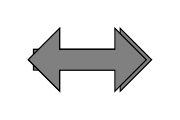
\begin{tikzpicture}
	\node [single arrow, draw,fill=gray,minimum height = 1.5cm,minimum width=0.8cm,visible on=<1>] {};
	\node [double arrow, draw,fill=gray,minimum height = 1.5cm,minimum width=0.8cm,visible on=<2->] {};
	\end{tikzpicture}
\end{column}
	\begin{column}{5cm}
	%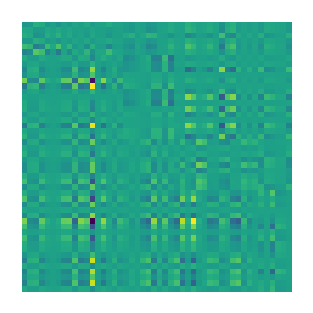
\includegraphics[width=\textwidth]{Plots/Matrix.pdf}
	%\includegraphics[width=\textwidth]{}
	%\vspace{-1cm}
	\begin{tikzpicture}
	\node[visible on=<1-2>] at (0,2) {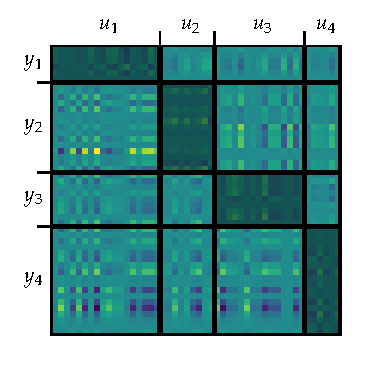
\includegraphics[width=\textwidth]{Plots/example_move.pdf}};
	\node[visible on=<3->] at (0,2) {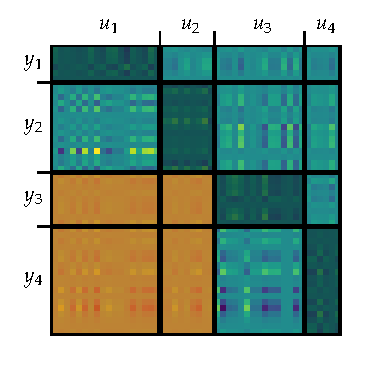
\includegraphics[width=\textwidth]{Plots/example_move_2.pdf}};
	%\draw (-3,0) rectangle (3,-2);
	\node[anchor = west,C1,visible on=<2->] (Hankel) at (0,-0.7) {Hankel matrix};
	\draw[->,C1,signal    ,visible on=<2->] (Hankel) to [out=180,in=270] (-0.7,0);
	\end{tikzpicture}
	\end{column}
	
\end{columns}
\end{frame}



\begin{frame}
	\frametitle{Approximation}
	\vspace{-1cm}
	\begin{tikzpicture}
	\node[] at (2,0) {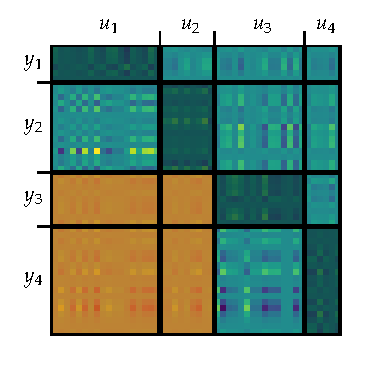
\includegraphics[width=3.5cm]{Plots/example_move_2.pdf}};
	%\draw (-3,0) rectangle (3,-2);
	\node[anchor = east,C1] (Hankel) at (-1,-0) {Hankel matrix};
	\draw[->,C1,signal    ] (Hankel) to [out=0,in=180] (0.5,-0.5);
	\end{tikzpicture}
	\begin{block}{State dimensions depend on Hankel matrices}
		$$\text{rank}(H_k) = \text{dim}(x_k)$$
	\end{block}
\pause
$ $\\
\textbf{Balanced Truncation:}\\
Remove states corresponding to small singular values
\end{frame}

\begin{frame}
	\begin{exampleblock}{Reseach Question}
		How do we choose the input and output dimensions?
	\end{exampleblock}
\end{frame}

\begin{frame}
	\chapterpage{Algorithms}
\end{frame}

\begin{frame}
\frametitle{Optimizing Input and Output Dimensions}
\begin{block}{Optimization Problem}
	\begin{itemize}
		\item Discrete optimization
		\item Objective function
	\end{itemize}
\end{block}
\end{frame}

\begin{frame}
	\frametitle{Algorithms}
	\begin{exampleblock}{A}
		Adapt initial dimensions
	\end{exampleblock}
	\pause
	\begin{exampleblock}{B}
		Recursive splitting
	\end{exampleblock}
\end{frame}

\begin{frame}
\frametitle{A: Change dimensions}
\scalebox{0.8}{\begin{tikzpicture}[font=\small,fontmatrices=\small,boxsize=11mm]
%violet!80!red!90
\tikzstyle{colmarking} = [magenta!50!violet!100,line width=1.5pt]
\def\colortext{magenta!50!violet!100}


\def\distorig{\rel_i_stage*\pgfkeysvalueof{/tikz/boxsize}}
\def\distvert{2.7mm}
%\def

	\matrix (m1) [row sep=5.mm, column sep=9mm] at (-3.2,0)
	{
		&		\node[coordinate]  (xin) {}; & \\[1.2cm,between origins]
		%--------------------------------------------------------------------
		\node[]                  (u_1) {$u_{k}$};          &
		\node[style_stage, stage, name=sys_1,A=$$,B=$$,C=$$,D=$$] {};&
		\node[]                  (y_1) {$y_k$};          \\
		%--------------------------------------------------------------------
		\node[]                  (u_2) {$u_{k+1}$};          &
		\node[style_stage, stage, name=sys_2,A=$$,B=$$,C=$$,D=$$] {};&
		\node[]                  (y_2) {$y_{k+1}$};          \\[1.4cm,between origins]

		 &		\node[coordinate]  (xout) {}; & \\
	};


	\foreach \i in {1,2}
		{
		  \draw[signalflow] (u_\i) -- (sys_\i.u);
	  	\draw[signalflow] (sys_\i.y) -- (y_\i);
		}
	\draw[signalflow] (xin)                      -- node[anchor = west]          {$x_{k}$} (sys_1.xin);
	\draw[signalflow] (sys_1.xout)               -- node[anchor=west]            {$x_{k+1}$} (sys_2.xin);
	\draw[signalflow] (sys_2.xout)               -- node[near end,anchor = west] {$x_{k+2}$} (xout);


%d-connection
\draw[signalflow, colmarking] (u_2) to [out=0,in=180] node[near end,anchor = south] {$u_\m$} ($(sys_2.u)+(0,+\distvert)$)-- ($(sys_2.center)+(-\distorig,+\distvert)$);
%\draw[signalflow, colmarking] ($(u_2.east)+(0,\distvert)$) --  ($(sys_2.u)+(0,\distvert)$);
\draw[signalflow,colmarking] ($(sys_2.u)+(0,\distvert)$)--node[anchor=south] {$d$} ($(sys_2.center)+(0.5*\distorig,\distvert)$);
 \draw[signal, colmarking] ($(sys_2.center)+(0.5*\distorig,\distvert)$) to [out=0,in=180] (sys_2.y);

%diagonal
 \draw[signalflow,colmarking,line cap=round] ($(sys_2.center)+(-\distorig,\distvert)$) -- node[name=b,pos = 0.5]   {} ($(sys_2.center)+(0,-\distorig+\distvert)$)  ;
%down
\draw[signal,colmarking] ($(sys_2.center)+(0,-\distorig+\distvert)$) -- (sys_2.xout);

\node (btext) at ($(sys_2.center)+(-\distorig,-\distorig)$) {$\;\textcolor{\colortext}{b}$};

\draw[white,line width=1mm,opacity=0.8] (btext) to [out=80,in=200] (b);
\draw[colmarking,line width=0.7pt] (btext) to [out=80,in=200] (b);



	\matrix (m1) [row sep=5.mm, column sep=9mm] at (3.2,0)
	{
		&		\node[coordinate]  (xin) {}; & \\[1.2cm,between origins]
		%--------------------------------------------------------------------
		\node[]                  (u_1) {$\tilde{u}_{k}$};          &
		\node[style_stage, stage, name=sys_1,A=$\tilde{A}_k$,B=$$,C=$$,D=$$] {};&
		\node[]                  (y_1) {${y}_{k}$};          \\
		%--------------------------------------------------------------------
		\node[]                  (u_2) {$\tilde{u}_{k+1}$};          &
		\node[style_stage, stage, name=sys_2,A=$$,B=$$,C=$$,D=$$] {};&
		\node[]                  (y_2) {${y}_{k+1}$};          \\[1.4cm,between origins]

		 &		\node[coordinate]  (xout) {}; & \\
	};


	\foreach \i in {1,2}
		{
		  \draw[signalflow] (u_\i) -- (sys_\i.u);
	  	\draw[signalflow] (sys_\i.y) -- (y_\i);
		}
	\draw[signalflow] (xin)                      -- node[anchor = west]          {$x_k$} (sys_1.xin);
	\draw[signalflow] (sys_1.xout)               -- node[anchor=west]            {$\tilde{x}_{k+1}$} (sys_2.xin);
	\draw[signalflow] (sys_2.xout)               -- node[near end,anchor = west] {$x_{k+2}$} (xout);


\draw[white,line width=2.5mm,opacity=0.8] ($(sys_2.center)+(-\distvert,\distorig)$) -- ($(sys_2.center)+(\distorig-\distvert,0)$)  ;

\draw[signalflow, colmarking] (u_1) to [out=0,in=180] node[near end,anchor = north] {$u_\m$} ($(sys_1.u)+(0,-\distvert)$)-- ($(sys_1.center)+(-\distorig,-\distvert)$);
 %\draw[signalflow, colmarking] ($(u_1.east)+(0,-\distvert)$) -- ($(sys_1.u)+(0,-\distvert)$);
 \draw[signal,colmarking,dotted] ($(sys_1.u)+(0,-\distvert)$)-- ($(sys_1.center)+(0.5*\distorig,-\distvert)$);
 \draw[signalflow, colmarking,dotted] ($(sys_1.center)+(0.5*\distorig,-\distvert)$)  to [out=0,in=180] node[anchor=north] {$d_{\text{new}}$} (sys_1.east);

%diag eye
\draw[signal,colmarking,line cap=round] ($(sys_1.center)+(-\distorig,-\distvert)$) --  ($(sys_1.center)+(-\distvert,-\distorig)$)  ;
\draw[signalflow,colmarking] ($(sys_1.center)+(-\distvert,-\distorig)$) -- ($(sys_2.center)+(-\distvert,\distorig)$);
%dia_d
\draw[signalflow,colmarking,line cap=round] ($(sys_2.center)+(-\distvert,\distorig)$) -- node[name=d]   {} ($(sys_2.center)+(\distorig-\distvert,0)$)  ;
\draw[signal,colmarking] ($(sys_2.center)+(\distorig-\distvert,0)$) -- (sys_2.y);
%back to x
\draw[signalflow,colmarking] ($(sys_2.center)+(-\distvert,\distorig)$)-- ($(sys_2.center)+(-\distvert,\distvert)$) to [out=270,in=90] node[name=b] {} ($(sys_2.center)+(-0,-\distorig)$) -- (sys_2.xout);
\node (btext) at ($(sys_2.center)+(-\distorig,-\distorig)$) {$\;\;\textcolor{\colortext}{b}$};
\node (dtext) at ($(sys_2.center)+(\distorig,\distorig)$) {$\!\textcolor{\colortext}{d}$};

\draw[white,line width=1mm,opacity=0.8] (btext) to [out=60,in=180] (b);
\draw[colmarking,line width=0.7pt] (btext) to [out=60,in=180] (b);

\draw[white,line width=1mm,opacity=0.8] (dtext) to [out=180,in=80] (d);
\draw[colmarking,line width=0.7pt] (dtext) to [out=180,in=80] (d);


\end{tikzpicture}
}
\end{frame}

\begin{frame}
	\frametitle{A: Objective Function}
	\begin{block}{Nuclear Norm}
		$$f =  \frac{\|T\|_*}{\|T\|}$$
		Convex hull of $\text{rank}(T)$
	\end{block}
	\begin{block}{Computational cost}
	$$f = \text{Number of multiplications}$$
	\end{block}
\end{frame}

\begin{frame}
	\frametitle{A: Optimize}
	\begin{tikzpicture}
	\node[visible on=<1>] at (0,0) {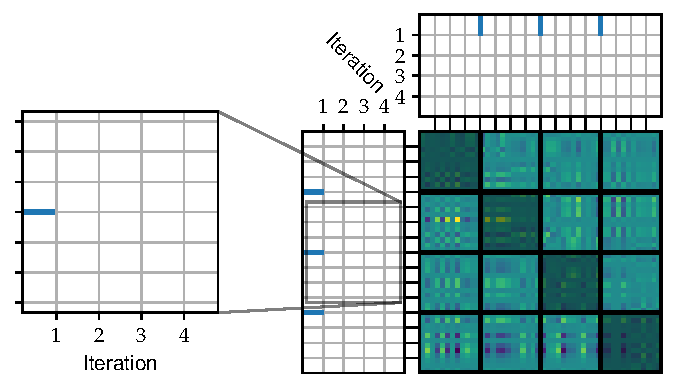
\includegraphics[width=0.8\textwidth]{Plots/example_move_iterations0.pdf}};
	\node[visible on=<2>] at (0,0) {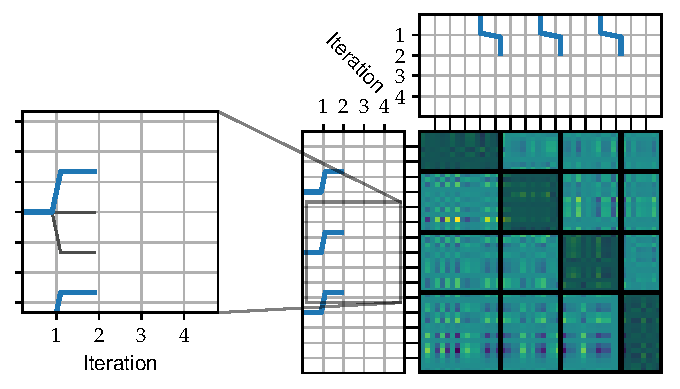
\includegraphics[width=0.8\textwidth]{Plots/example_move_iterations1.pdf}};
	\node[visible on=<3>] at (0,0) {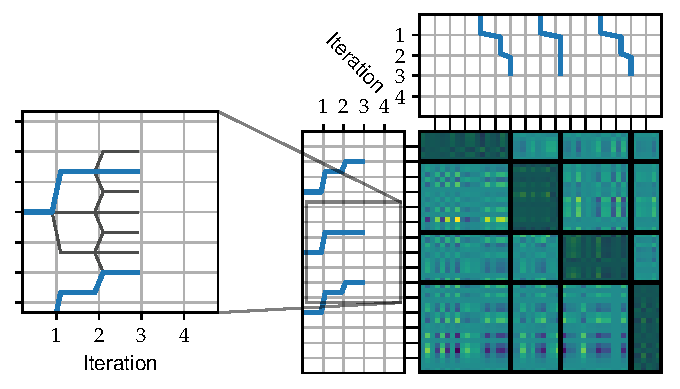
\includegraphics[width=0.8\textwidth]{Plots/example_move_iterations2.pdf}};
	\node[visible on=<4>] at (0,0) {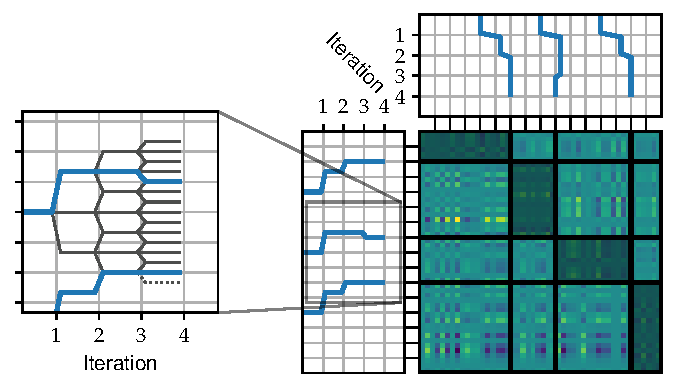
\includegraphics[width=0.8\textwidth]{Plots/example_move_iterations3.pdf}};
	\node[visible on=<5>] at (0,0) {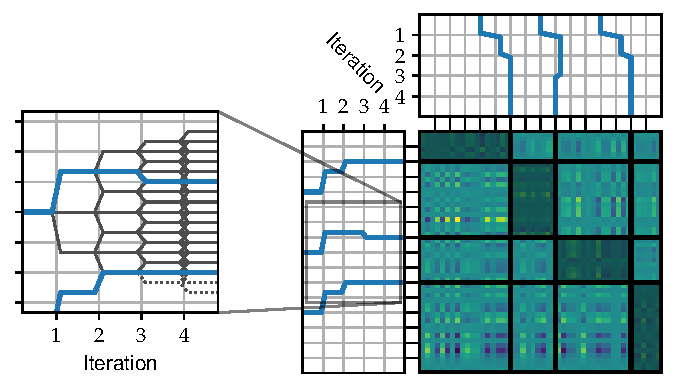
\includegraphics[width=0.8\textwidth]{Plots/example_move_iterations4.pdf}};
	\end{tikzpicture}
\end{frame}

\begin{frame}
	\frametitle{Algorithms}
	\begin{exampleblock}{A}
		Adapt initial dimensions
	\end{exampleblock}
	\begin{exampleblock}{B}
		Recursive splitting
	\end{exampleblock}
\end{frame}

\begin{frame}
	\frametitle{B: Permutation of Columns and Rows}
	\centering
	\scalebox{0.8}{\begin{tikzpicture}[font=\small,fontmatrices=\small,boxsize=6.5mm,distconn=0.85]


\tikzset{per/.style={rectangle,draw=black!50,fill=black!20,thick,inner sep=0pt,minimum size=12.5mm}}

	\matrix (m1) [row sep=3.mm, column sep=10mm]
	{
		&&		\node[coordinate]  (xin) {}; & \\[0.7cm,between origins]
		%--------------------------------------------------------------------
		\node[]                  (u_1) {$u_1$};          &
		\node[per]               (pl1) { };&
		\node[style_stage, stage, name=sys_1,A=$$,B=$$,C=$$,D=$$] {};&
		\node[per]               (pr1) { };&
		\node[]                  (y_1) {$y_1$};          \\
		%--------------------------------------------------------------------
		\node[]                  (u_2) {$u_2$};          &
		\node[per]               (pl2) { };&
		\node[style_stage, stage, name=sys_2,A=$$,B=$$,C=$$,D=$$] {};&
		\node[per]               (pr2) { };&
		\node[]                  (y_2) {$y_2$};          \\[1.1cm,between origins]
		%--------------------------------------------------------------------
		\node[anchor=mid]  (dots_u) {$\mathbf{\vdots}$}; &&
		\node[anchor=mid]  (dots_x) {$\mathbf{\vdots}$}; &&
		\node[anchor=mid]  (dots_y) {$\mathbf{\vdots}$}; \\[0.9cm,between origins]
		%--------------------------------------------------------------------
		\node[]                  (u_k) {$u_K$};          &
		\node[per]               (plk) { };&
		\node[style_stage, stage, name=sys_k,A=$$,B=$$,C=$$,D=$$] {};&
		\node[per]               (prk) { };&
		\node[]                  (y_k) {$y_K$};          \\[0.7cm,between origins]
		%--------------------------------------------------------------------
		 &&		\node[coordinate]  (xout) {}; & \\
	};



	\foreach \i in {1,2,k}
		{
		  \draw[signalflow] (u_\i) -- (pl\i);
	  	\draw[signalflow] (pl\i) -- (sys_\i.u);
		  \draw[signalflow] (sys_\i.y) -- (pr\i);
     \draw[signalflow] (pr\i) -- (y_\i);
		}
	\draw[signalflow] (xin)                      -- node[anchor = west]          { } (sys_1.xin);
	\draw[signalflow] (sys_1.xout)               -- node[anchor=west]            { } (sys_2.xin);
	\draw[signalflow,posarr=0.8] (sys_2.xout)               -- node[near end,anchor=west]   { } ($(dots_x.north)+(0,-0.1)$);
	\draw[signalflow,posarr=0.6] ($(dots_x.south)+(0,-0.0)$) -- node[near start,anchor=west] { }(sys_k.xin);
	\draw[signalflow,posarr=0.7] (sys_k.xout)               -- node[near end,anchor = west] { } (xout);

\draw[style_stage] (pl1.north west) rectangle (plk.south east);
\draw[style_stage] (pr1.north west) rectangle (prk.south east);

\node (Pi) at ($(pl1.north)!0.5!(plk.south)$) {$\Pi_i$};
\node (Pi) at ($(pr1.north)!0.5!(prk.south)$) {$\Pi_o$};
\end{tikzpicture}}
\end{frame}

\begin{frame}
	\frametitle{B: Spiting Stage}
	\scalebox{0.8}{\begin{tikzpicture}[font=\small,fontmatrices=\small,boxsize=6.5mm,distconn=0.85]
%violet!80!red!90
%\tikzstyle{colmarking} = [C0,line width=1.5pt]
%\def\colortext{magenta!50!violet!100}


\def\distorig{\rel_i_stage*\pgfkeysvalueof{/tikz/boxsize}}
\def\distvert{2.7mm}
%\def


\def\distorigb{1.4*\distorig}

	\matrix (m1) [row sep={1.5cm,between origins}, column sep={2.3cm,between origins}] at (-3.2,0) %col 2.5
	{
		&		\node[coordinate]  (xin) {}; & \\[0.4cm,between origins]
		%--------------------------------------------------------------------
		\node[]                  (u) {$u_{k}$};          &
		\node[style_stage, stage, name=sys,boxsize=11mm,distconn=0.65] {};&
		\node[]                  (y) {$y_{k}$};          \\[0.4cm,between origins]

		 &		\node[coordinate]  (xout) {}; & \\
	};
	\node[shape=rectangle,minimum size=2*11mm] (sys_a) at (sys) {};
	\draw[signalflow] (u) -- (sys_a.west);
	\draw[signalflow] (sys_a.east) -- (y);
	\draw[signalflow] (xin)                      -- node[anchor = west]          {$x_{k}$} (sys_a.north);
	\draw[signalflow] (sys_a.south)                -- node[anchor=west]            {$x_{k+1}$} (xout);

%split in
%\draw[signalflow,posarr=0.7] (u) to [out=0,in=180] node[anchor = south] {$u_\alpha\quad$} ($(sys_a.west)+(0,+\distvert)$);
%\draw[signalflow,posarr=0.7] (u) to [out=0,in=180] node[anchor = north] {$u_\beta\quad$} ($(sys_a.west)+(0,-\distvert)$);

%split out
%\draw[signalflow,posarr=0.3] ($(sys_a.east)+(0,+\distvert)$) to [out=0,in=180] node[anchor = south] {$y_\alpha$} (y);
%\draw[signalflow,posarr=0.3] ($(sys_a.east)+(0,-\distvert)$) to [out=0,in=180] node[anchor = north] {$y_\beta$} (y);




\tikzset{per/.style={rectangle,draw=black!50,fill=black!20,thick,inner sep=0pt,minimum height=12.5mm,minimum width=8.5mm}}

	\matrix (m1) [row sep=3.mm, column sep=5mm] at (3.2,0)
	{
		&&		\node[coordinate]  (xin) {}; & \\[0.7cm,between origins]
		%--------------------------------------------------------------------
		\node[]                  (u_1) {$u_1$};          &
		\node[per]               (pl1) { };&
		\node[style_stage, stage, name=sys_1,A=$$,B=$$,C=$$,D=$$] {};&
		\node[per]               (pr1) { };&
		\node[]                  (y_1) {$y_1$};          \\
		%--------------------------------------------------------------------
		\node[]                  (u_2) {$u_2$};          &
		\node[per]               (pl2) { };&
		\node[style_stage, stage, name=sys_2,A=$$,B=$$,C=$$,D=$$] {};&
		\node[per]               (pr2) { };&
		\node[]                  (y_2) {$y_2$};          \\[0.7cm,between origins]
		%--------------------------------------------------------------------
		 &&		\node[coordinate]  (xout) {}; & \\
	};



	\foreach \i in {1,2}
		{
		  \draw[signalflow] (u_\i) -- (pl\i);
	  	\draw[signalflow] (pl\i) -- (sys_\i.u);
		  \draw[signalflow] (sys_\i.y) -- (pr\i);
     \draw[signalflow] (pr\i) -- (y_\i);
		}
	\draw[signalflow] (xin)                      -- node[anchor = west]          { } (sys_1.xin);
	\draw[signalflow] (sys_1.xout)               -- node[anchor=west]            { } (sys_2.xin);
	\draw[signalflow,posarr=0.7] (sys_2.xout)    -- node[near end,anchor = west] { } (xout);

\draw[style_stage] (pl1.north west) rectangle (pl2.south east);
\draw[style_stage] (pr1.north west) rectangle (pr2.south east);

\node (Pi) at ($(pl1.north)!0.5!(pl2.south)$) {$\Pi_i$};
\node (Pi) at ($(pr1.north)!0.5!(pr2.south)$) {$\Pi_o$};\end{tikzpicture}
}
\end{frame}

\begin{frame}
	\frametitle{B: Partition inputs and outputs}
	\makeatletter
\DeclareRobustCommand{\rvdots}{%
  \vbox{
    \baselineskip4\p@\lineskiplimit\z@
    \kern-\p@
    \hbox{.}\hbox{.}\hbox{.}
  }}
\makeatother

\tikzstyle{border} = [line width=0.8pt]%[very thick]


\begin{equation}
	\begin{bmatrix}\begin{tikzpicture}
     \matrix [%
       matrix of math nodes,
       column sep=0em,
       row sep=0.8em,
     ] (y) {%
				x^*_{k-1}\\
       y_{k} \\
       x_{k+1}\\
     };

		\node[name=s_line,shape=coordinate] at ($(y-1-1.west)!0.5!(y-3-1.west)$) {};
		\draw[border,C0] (s_line) -- ($(s_line)!(y-3-1.east)!($(s_line)+(1,0)$)$);

     \matrix [%
       matrix of math nodes,
       column sep=0em,
       row sep=0.8em,
     ] (y) {%
				x^*_{k-1}\\
       y_{k} \\
       x_{k+1}\\
     };
   \end{tikzpicture} \end{bmatrix}
=
\begin{matrix}\begin{tikzpicture}
     \matrix [%
       matrix of math nodes,
       column sep=0.8em,
       row sep=0.7em,
				left delimiter=\lbrack,right delimiter=\rbrack
     ] (T) {
%	0   &B_k^* & B_k^*& A_k^*\\
%	C_k & D_k & D_k &C_k^*\\
%  C_k & D_k & D_k &C_k^*\\
%	A_k & B_k &B_\beta & 0 \\
	0   &B_k^* & A_k^*\\
	C_k & D_k & C_k^*\\
	A_k & B_k & 0 \\
     };

\filldraw[name = Hrect, fill=C0!40, draw=white] (T-2-1.west) rectangle  ($(T-3-2.south)-(0.15em,0)$); 
\filldraw[name = Harect,fill=C0!40, draw=white] (T-2-3.east) rectangle  ($(T-1-2.north)-(0.15em,0)$); 
\draw[border,C0] (T-2-1.west) -- (T-2-3.east);
\draw[border,C0] ($(T-1-2.north)-(0.15em,0)$) -- ($(T-3-2.south)-(0.15em,0)$);

     \matrix [%
       matrix of math nodes,
       column sep=0.8em,
       row sep=0.7em
     ] (T) {
%	0   &B_k^* & B_k^*& A_k^*\\
%	C_k & D_k & D_k &C_k^*\\
%  C_k & D_k & D_k &C_k^*\\
%	A_k & B_k &B_\beta & 0 \\
	0   &B_k^* & A_k^*\\
	C_k & D_k & C_k^*\\
	A_k & B_k & 0 \\
     };

\node[name=Hcausakpos,shape=coordinate] at ($(T-3-1.south east)+(-0.2em,-1em)$) {};
\node[anchor = east,C0] (Hcausal) at (Hcausakpos) {$H$};
\draw[->,C0,border] ($(Hcausakpos)+(-1.5mm,0)$) to [out=0,in=270] (T-3-1.south east);
\node[name=Hanticausakpos,shape=coordinate] at ($(T-1-3.north west)+(0.2em,1.35em)$) {};
\node[anchor = west,C0] (Hanticausal) at (Hanticausakpos) {$H^*$};
\draw[->,C0,border] ($(Hanticausakpos)+(1.5mm,0)$) to [out=180,in=90] (T-1-3.north west);

\end{tikzpicture} 
\end{matrix}
	\begin{bmatrix}\begin{tikzpicture}
     \matrix [%
       matrix of math nodes,
       column sep=0em,
       row sep=0.9em,
     ] (u) {%
				x^*_{k}\\
       u_{k} \\
       x_{k}\\
     };
		\node[name=s_line,shape=coordinate] at ($(y-1-1.west)!0.5!(y-3-1.west)$) {};
		\draw[border,C0] (s_line) -- ($(s_line)!(y-3-1.east)!($(s_line)+(1,0)$)$);

     \matrix [%
       matrix of math nodes,
       column sep=0em,
       row sep=0.9em,
     ] (u) {%
				x^*_{k}\\
       u_{k} \\
       x_{k}\\
     };
   \end{tikzpicture} \end{bmatrix}
\end{equation}



\end{frame}

\begin{frame}
	\frametitle{B: Optimize}
	\centering
	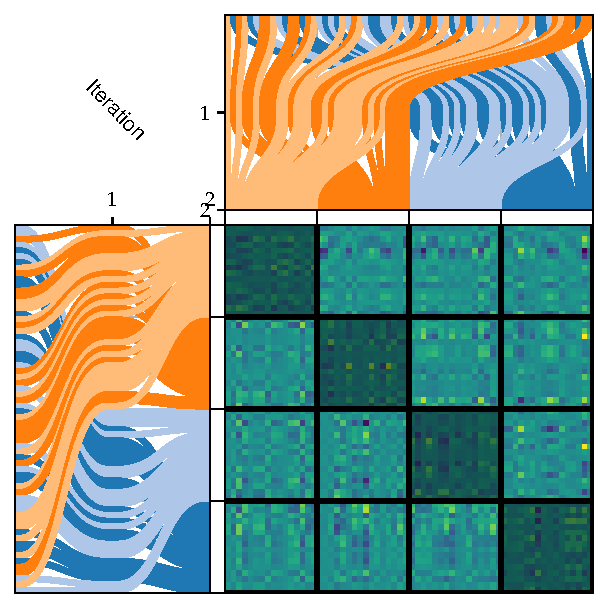
\includegraphics[width=0.6\textwidth]{../Thesis/Plots/example_permute.pdf}
\end{frame}

\begin{frame}
	\chapterpage{Is it useful?}
\end{frame}

\begin{frame}
	\frametitle{Adaptation for Neural Net Weight matrix}
	\centering
	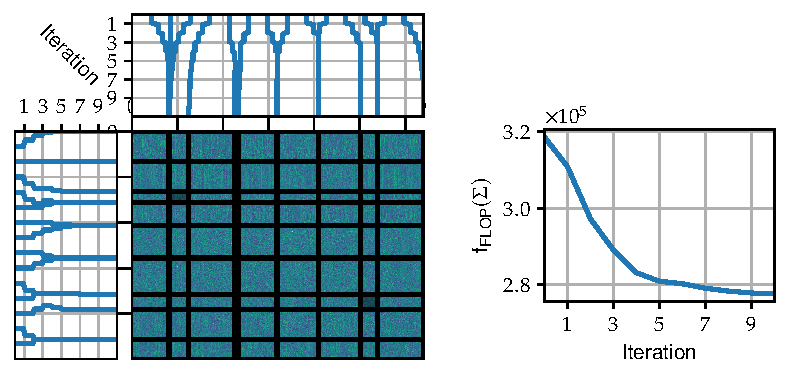
\includegraphics[trim=0cm 0cm 6cm 0cm, clip,width=0.6\textwidth]{../Thesis/Plots/move_example_mobilenet_comp.pdf}
\end{frame}

\begin{frame}
	\frametitle{Approxiamtion}
	\centering
	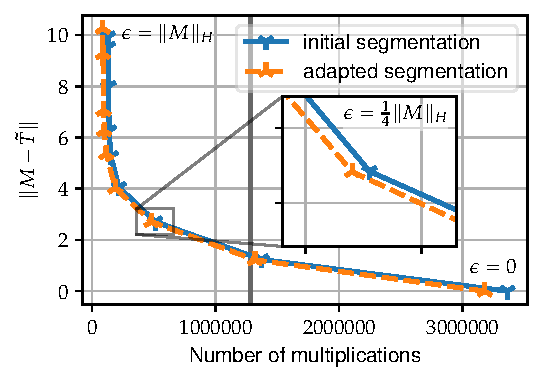
\includegraphics[width=0.7\textwidth]{../Thesis/Plots/move_example_mobilenet_error.pdf}
\end{frame}

\begin{frame}
	\frametitle{Permutation for Neural Net Weight matrix}
	\centering
	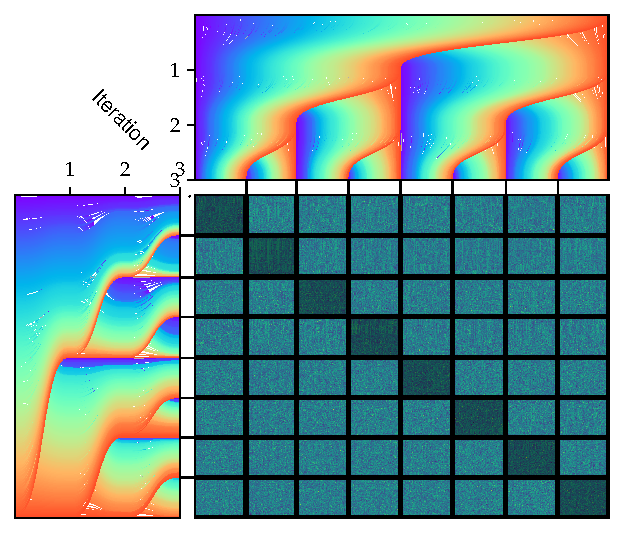
\includegraphics[width=0.6\textwidth]{../Thesis/Plots/Mobilenet_permute.pdf}
\end{frame}

\begin{frame}
	\frametitle{Approxiamtion}
	\centering
	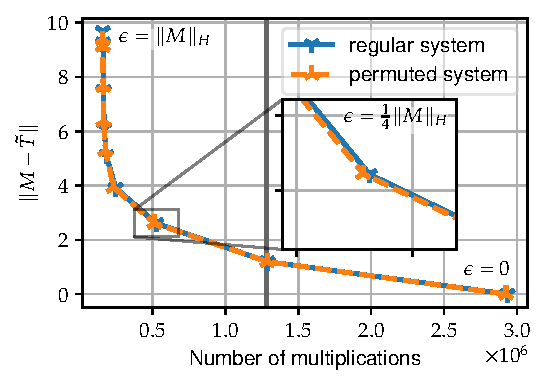
\includegraphics[width=0.7\textwidth]{../Thesis/Plots/perm_example_mobilenet_error.pdf}
\end{frame}

\begin{frame}
	\chapterpage{What does this mean?}
\end{frame}


\begin{frame}
	Algorithms were not able to extract a clear structure from the matrix
	
	\pause
	\begin{block}{Result}
	Algorithm A is able to reduce the computational cost without increasing the approximation error
	\end{block}

\end{frame}





\section{Blocks \& Math}
\subsection{Blocks}
\begin{frame}
   \frametitle{Blocks}

   \begin{block}{This is a simple block}
      It should contain some text.
   \end{block}

   \begin{exampleblock}{Example Block}
      This may be an example.
   \end{exampleblock}


   \begin{alertblock}{Warning}
      The violent color indicates that this block may alert of something.
   \end{alertblock}
\end{frame}


\end{document}
